\cotefile{18}
\scanpage{2}
\unsure{Papiers|Papier} donnés à Saavedra
% archive sheet number: 1

\scanpage{3}
\mspage{Page 6}

Proposal to National Science Foundation

7. The Existence and Unicity of Best Approximations (with E.W. Cheney), \uline{Math. Scand.}, (To Appear, Summer 1969).

8. Convergence of Operators and Korovkin's Theorem, \uline{J. of Approx. Theory}, \uline{1}, (1968), pp. 381-390.

9. Continuous Selections for Metric Projections (with A.J. Lazar and P.D. Morris), \uline{J. of Funct. Analy.}, \uline{3}, (1968), pp. 193-216.

10. A characterization of $C(X)$ for $X$ locally connected. \uline{Proc. Amer. Math. Soc.}, \uline{21}, (1969), pp. 269-272.

11. On the Minimal Property of the Fourier Projection (with E.W. Cheney, C.R. Hobby, P.D. Morris and F. Schurer), \uline{Trans. Amer. Math. Soc.}, (To Appear).

12. The classification of Banach spaces whose duals are $L_{1}$ spaces (with J. Lindenstrauss). \uline{J. of Funct. Analy.}, (To Appear).

13. In Preparation. ``Characterizations of Conditional Expectations.''

RESEARCH ANNOUNCEMENTS

14. Structure of Tchebychev sets, \uline{Proc. of the Second Symposium on General Topology and its Applications to Modern Analysis and Algebra}, Prague, 1966, pp. 356-359. This paper is an announcement of (4) above.

15. Locally connected Stone-Cech compactifications, \uline{Proc. of First International Symposium on Extension Theory of Topological Structures and its Applications} (To Appear). This paper is an announcement of (10) above.

16. On the minimal property of the Fourier Projection (with E.W. Cheney, C.R. Hobby, P.D. Morris and F. Schurer), \uline{Bull. Amer. Math. Soc.}, \uline{75}, (1969), pp. 51-52. This is an announcement of (11) above.
% archive sheet number: 2

\scanpage{4}
\uline{Motifs et cristaux} \uline{sur corps local}
% archive sheet number: 3

\scanpage{5}
Descriptions conjecturales des motifs sur corps de nbs \deleted{\unsure{$F$|$K$}} $k$

1) Double réseau Betti-De Rham

2) Double réseau Betti-Hodge

3) \deleted{Betti + \unsure{bigradé|bigrad.}} structure de Hodge $(k=\overline{\unsure{Q|\mathbb Q}})$

4) \deleted{Betti + \unsure{connexion} réseau Betti} Betti-(Gauss)Manin $(k=\overline Q)$

5) \deleted{Tate} Betti-Tate

6) \deleted{De Rham - cristal} De Rham filtré cristallin

Descriptions conjecturales des groupes $p$-divisibles \inserted{mod isogénie} (plus \unsure{génér\textsuperscript{t}|génér\textsuperscript{alt}|gén.} des pseudo-motifs) sur un corps local [\deleted{\unsure{spectre}} \inserted{corps de fr.} d'un ann. de val. discrète complet à corps rés \deleted{\unsure{parfait}}] :

$3'$) structure de Hodge-\inserted{Tate\unsure{;|:} module $N$ de t.f. sur $Q_p$, et bigrad. sur $N\otimes_{\unsure{Q_p|Q|\mathbb Q_p}} C$} (mod ext. finie de $K$)

$2'$) double réseau Tate-Hodge

$5'$) Tate (module galoisien $\unsure{l|\ell}$-adique)

$6'$) \deleted{\unsure{module de vect. de Di|module vect. de Di|module Vect. de di}} cristal filtré [vectoriel \deleted{\unsure{sur}} dim finie sur $K$, une application $\sigma$-semi-linéaire, \deleted{\unsure{et|+}} filtration, graduation]

Par quoi remplacer $1',4'$ ??
% archive sheet number: 4

\scanpage{6}
\diagram{\begin{tikzcd}[ampersand replacement=\&,row sep=small,column sep=small]
\& \pi \arrow[d,"u"'] \\
\& G(\unsure{Q|\mathbb Q}_p) \arrow[d,phantom,"\rotatebox{270}{$\subset$}" description] \\
\& G(C) \arrow[d,phantom,"\unsure{\wr\vert|\simeq|j_1}" description] \\
1 \arrow[r,dash] \& G'(C) \arrow[r] \arrow[d,phantom,"\rotatebox{90}{$\subset$}" description] \& E \arrow[r] \& \pi \arrow[l,bend right=32,"\sigma_1"'] \arrow[l,bend left=32,"\sigma_2"] \arrow[r,dash] \& 1 \\
\& G'(Q_p) \\
\& G_m(Q_p)=Q_p^* \arrow[u,hook,"j_2"] \\
\& \pi \arrow[u,"\chi"]
\end{tikzcd}}

\deleted{\unsure{$\alpha$}} $\alpha$ permet d'identifier une certaine ext. de $E$ de $\pi$ par $G'(C)$ avec une \deleted{autre} ext. de $\pi$ par $G(C)$

Le splitting $\sigma_2$ de la première est tel que $\sigma_2(\pi)$ commute à $G'(Q_p)$ et a fortiori à $j_2\chi(\pi)$. On trouve donc
\[
\left\{\begin{aligned}
\gamma&\longmapsto\widetilde{\sigma}_2(\gamma)=\sigma_2(\gamma).j_2(\chi(\gamma))\\
\pi&\longrightarrow E
\end{aligned}\right.
\]
un autre splitting.

Le splitting $\sigma_1$ \deleted{\unsure{de|dans}} la seconde commute à $G(Q_p)$, et à fortiori à $u(\pi)$. On \deleted{trouve donc}
\[
\gamma\longmapsto\sigma_1(\gamma)u(\gamma)=\widetilde{\sigma}_1(\gamma)
\]

On écrit que $\widetilde{\sigma}_1(\gamma)=\widetilde{\sigma}_2(\gamma)$

\margin{\unsure{$\lrcorner$|1}}% margin note written sideways
i.e.
\[
\sigma_2(\gamma)\,j_2(\chi(\gamma))=\sigma_1(\gamma)\,u(\gamma)
\]
donc
\[
\underbrace{\sigma_1(\gamma)^{-1}\sigma_2(\gamma)}_{\varphi(\gamma)}
=\deleted{\unsure{j_2}}\underset{\substack{\rotatebox{270}{$\in$}\\G(Q_p)}}{u(\gamma)}\mathord{.}
\underset{\substack{\rotatebox{270}{$\in$}\\j_2(Q_p^*)}}{\underline{j_2(\chi(\gamma^{-1}))}}
\]

1\textsuperscript{o}) Sur $\operatorname{Ker}\chi$, on a $\varphi(\gamma)=u(\gamma)$. donc $u$ connu sur $\operatorname{Ker}\chi$

2\textsuperscript{o}) $\operatorname{Ker}u=\deleted{\chi(\gamma)}\{\gamma,\chi(\gamma)=1,\varphi(\gamma)=1\}$ connu. Soit $\Pi_1=\pi/\operatorname{Ker}u$. C'est un gpe analytique $p$-adique, et $\Pi_1\xrightarrow{\chi_1}Q_p^{\unsure{*|1}}$ induit par $p$
% archive sheet number: 5

\scanpage{7}
\mspage{\handwritten{18}}
\diagram{\[
\begin{tikzcd}[ampersand replacement=\&]
\mathrm{Gr}^{\handwritten{i}}(X_{\bar t})_{\handwritten{\mathbb Q}}
 \handwritten{\arrow[r,"{\mathrm{cl}}"]\arrow[d]} \&
 H^{2i}(X_{\bar t},\underline{Q}_{\unsure{l|\ell}}(i))
 \handwritten{\arrow[d,"\wr"]}\\
\mathrm{Gr}^{\handwritten{i}}(X_{\bar s})_{\handwritten{\mathbb Q}}
 \handwritten{\arrow[r,"{\mathrm{cl}}"]} \&
 H^{2i}(X_{\bar s},\underline{Q}_{l}(i))\;.
\end{tikzcd}\tag*{(7.13.10\deleted{\unsure{9}}\handwritten{)}}
\]}

\deleted{7.13.11.} \uline{Remarque\deleted{s}} 7.13.11. La commutativité des deux derniers diagrammes \deleted{commutatifs}, qu'on peut exprimer en disant que la spécialisation des cycles \unsure{algébriqes|algébriques} est compatible avec la formation des classes de cohomologie $l$-adiques as\unsure{\^{s}|s}ociées, n'est pas très satisfaisante sous la forme énoncée, puisqu'on \deleted{\unsure{ne}} a été obligé de remplacer les coéfficients $\underline{\mathbb Z}_{l}(i)$ par $\underline{Q}_{l}(i)$, c'est à dire de négliger la torsion. Pour avoir un énoncé qui ne néglige pas la torsion, \deleted{on est}\inserted{il semble qu'on sera} obligé de travailler avec l'anneau de Chow, puisque c'est sur ce dernier que ce trouve défini naturellement l'homomorphisme $\mathrm{cl}$ comme homomorphisme à valeurs dans $H^{2*}(-,\underline{Z}_{l}(\unsure{*|i}))$, \deleted{\unsure{Malheureusement,}} comparer (XIV 4.1). Malheureusement, on n'a pas développé pour le moment une théorie de la spécialisation pour l'anneau de Chow\deleted{\unsure{,}} (cf. 7.1\deleted{\unsure{5|3}}\handwritten{4}), qui permettrait d'écrire \deleted{un diagramme}\inserted{des carrés} \deleted{\unsure{a}}commutatifs analogues à (7.13.9) et (7.13.10) en termes des anneaux de Chow et de la cohomologie à coéfficients $\underline{Z}_{l}(*)$. Tout ce qu'on peut dire\inserted{\handwritten{ lorsque $f:X\longrightarrow S$ est lisse et propre\unsure{,}}}, c'est qu'on a un carré commutatif
\diagram{\[
\begin{tikzcd}[ampersand replacement=\&]
Z^i(X_t) \handwritten{\arrow[r,"{\mathrm{cl}}"]\arrow[d,"\sigma"']} \&
 H^{2i}(X_t,\underline{Z}_{l}(i)) \handwritten{\arrow[d,phantom,"{\deleted{\downarrow}}" description,near end]}\\
Z^i(X_s) \handwritten{\arrow[r,"{\mathrm{cl}}"]} \&
 H^{2i}(X_s,\underline{Z}_{l}(i))\handwritten{\arrow[u]}\;,
\end{tikzcd}\tag*{(7.13.12)}
\]}
\deleted{et un carré} analogue à (7.13.9), et un carré correspondant analogue à (7.13.10) qu'on laisse au\deleted{\unsure{tre|x}} lecteur \inserted{\handwritten{le soin}} d'écrire, où $Z^i$ désigne le groupe des cycles algébriques (modulo rien du tout) de codimension $i$, \deleted{et} où les flêches horizontales sont les homomorphismes ``classe de cohomologie associée'' définie dans (SGA 5 IV), et où $\handwritten{\sigma}$ désigne l'homomorphisme de spécialisation des cycles algébriques, associant à un cycle $Z_t$ le cycle $Z_s$, où $Z$ est
% archive sheet number: 6

\scanpage{9}
\uline{Twist de Tate sur structures} \uline{de Hodge mixtes}

Soit $\unsure{\mathcal E|\mathscr E}\unsure{=|:}(E,E_0,\underset{\inserted{\text{croiss}}}{W_*^{\deleted{\unsure{*}}}},\underset{\inserted{\text{décr.}}}{F^*})$ une structure de Hodge mixte

On définit une structure de Hodge $\mathcal E(-1)$ \deleted{$=\unsure{\mathcal E(+1)|\mathcal E(1)}$,} (twist de Tate \inserted{effectif}) ; \deleted{\unsure{par}} avec même $E_0$ \deleted{espace vectoriel sur $Q$}\inserted{module sur $Z$}, donc même $E$,
\[
\left\{\begin{aligned}
W_i(\mathcal E(-1))&=W_{i\deleted{\unsure{+}}-2}(\mathcal E)\\
F^i(\mathcal E(-1))&=F^{i-1}(\mathcal E)
\end{aligned}\right.
\]

On trouve alors que
\[
 W_i(\mathcal E(-1)/W_{i-1}(\mathcal E(-1))\simeq
 [W_i(\mathcal E)/W_{i-1}(\mathcal E)](-1)
\]
(twist de Tate sur structures de Hodge ordinaires).

Bien \unsure{sur|sûr}, on définit pour tt entier $n$ un twist $\mathcal E(n)$,
\[
\left\{\begin{aligned}
W_i(\mathcal E(n))&=W_{i+2n}(\mathcal E)\\
F^i(\mathcal E(n))&=F^{i+n}(\mathcal E)
\end{aligned}\right.
\]
% archive sheet number: 8

\scanpage{10}
degrés de transcendance liés aux filtrations et bigraduations (comparaison de Betti, De Rham, Hodge)
% archive sheet number: 9

\scanpage{11}
\[
G''\supset H''\quad{}^{Q}H'\subset G'\quad{}^{P}G_k
\qquad
\boxed{\begin{aligned}
\alpha&\in P(\mathbb C)\\
\beta&\in Q(\mathbb C)\subset P'(\mathbb C)\\
\gamma&\in \deleted{\unsure{R}}P''(\mathbb C)
\end{aligned}}
\qquad
\begin{aligned}
\beta\alpha&=\gamma^{-1}\\
\gamma\beta&=\alpha^{-1}\\
\alpha\gamma&=\beta^{-1}
\end{aligned}
\]
\[
\left.\begin{aligned}
P&=\underline{\mathrm{Isom}}(T_B\otimes k,T_{\mathrm{DR}})\\
Q\subset P'&=\underline{\mathrm{Isom}}(T_{\mathrm{DR}},T_{\mathrm{Hdg}})\simeq Q\mathbin{\overset{H'}{\times}}G'\\
P''&=\underline{\mathrm{Isom}}(T_{\mathrm{Hdg}},T_B\otimes k)
\end{aligned}\right\}\text{ déf}/k
\]
\diagram{\begin{tikzcd}[ampersand replacement=\&,column sep=small]
\& T_{\mathrm{Hdg}}\otimes_k\mathbb C\arrow[dr,"\gamma"] \&\\
T_{\mathrm{DR}}\otimes_k\mathbb C\arrow[ur,"\beta"] \& \& T_B\otimes_{Q}\mathbb C\arrow[ll,"\alpha"]
\end{tikzcd}}

\[
\underbrace{U'}_{\substack{\text{rad.}\\\text{unipotent}\\\text{de }\unsure{U'|B'}}}
\subset\underbrace{B'}_{\substack{\text{parabolique}\\\text{associé à la}\\\text{filtration de}\\T_{\mathrm{DR}}}}\subset G'
\]
$Q=$ fibré des sous groupes de Lévi de $B'$
\[
 B'/U'\simeq L'\xleftarrow[\substack{\text{hom}\\\text{central}\\(\mathrm{Tate})}]{j'}G_m
\]

\[
\left.\begin{aligned}
\mathrm{Fil}&=\underline{\mathrm{Filt}}_{\substack{\otimes,\,\text{dans }\deleted{\unsure{\mathcal F}}\\
\text{classe int. de}\\\text{la filtration}\\\text{de }T_{\mathrm{DR}}}}\;T_{\unsure{b|B}}\\
\mathrm{Big}&=\underline{\mathrm{Bigr}}_{\substack{\otimes,\,\text{dans}\\\text{classe int de}\\
\text{la }\deleted{\unsure{\text{filtr.}}}\text{bigraduation}\\\text{de }T_{\mathrm{DR}}}}\;T_B
\end{aligned}\right\}\text{ déf}/Q
\]
\margin{$\nwarrow$ NB Soit $F\supset\mathrm{Fil},\Phi\supset\mathrm{Big}$ définis comme ci-contre, mais sans condition de forme intérieure. Alors $G$ y opère, et $A=F/G,B=\Phi/G$ sont des schémas \uline{\unsure{indét.|étales}} sur $Q$. Alors $\varphi\in F(\mathbb C),\psi\in\Phi(\mathbb C)$ \deleted{\unsure{définissent}} des pts $\dot\varphi\in A(\mathbb C),\dot\psi\in B(\mathbb C)$. \deleted{\unsure{$k$}} Soient $\varphi_1\in A,\psi_1\in B$ leurs images dans $A$ et $B$ (\unsure{pts} fermés \unsure{induits|susdits}) Par définition, $\mathrm{Fil}=F_{\varphi_1},\mathrm{Big}=\Phi_{\psi_1}$}
\margin{\uline{NB} Si on a $\varepsilon:\deleted{\unsure{\mathrm{Soit}}}G\longrightarrow G_m$ on a $(\varepsilon|(B'/U'))\circ j=\mathrm{id}.$ donc $j$ \unsure{mon.} Si $H'\subset B'$ est l'image inverse de $\operatorname{Im}j'$ dans $B'$, \deleted{\unsure{le tore}} $j'$ est \inserted{donc} connu quand on connait $H'$}

\[
P\times P'\longrightarrow P'',\quad P'\times P''\unsure{\mathbin{-}|\longrightarrow}P,\quad
P''\times P\longrightarrow P',\qquad Q\subset P'
\]

$\mathrm{Big}\xrightarrow[\deleted{\unsure{d}}]{p}\mathrm{Fil}$ fibration, faisant de $B$ un torseur sur $\mathrm{Fil}$, de groupe $U_{\mathrm{Fil}}$, un groupe unipotent défini sur $F$, de dim. relative égale à $\dim U'$. $\mathrm{Fil}$ est \unsure{des|de} dim égale à $\dim G'/B'$, $\mathrm{Big}$ est de dim égale à $\dim G'/B'+\dim U'=\dim G'/L'$, où $L'\deleted{\unsure{=}}=\operatorname{Centr}(j'_0)$, $j'_0:G_m\xrightarrow[k]{}H'$ relevant $j'$.

\margin{en fait, $\dot\varphi,\dot\psi$ sont dans $A(k),B(k)$ donc dans $A(k_1),B(k_1)$, où $k_1$ est la clôture alg. de $Q$ dans $k$. D'ailleurs, \deleted{$F\longrightarrow\Phi$ \unsure{induit}} $A\xrightarrow{\sim} B$, donc}
\margin{\unsure{constr.} explicite en termes du groupe déployé, associé au réseau \unsure{cor.} $\Gamma$ avec $W$ (Weyl) agissant : on \unsure{tord|aura} $\Gamma/W$ par autom. extérieurs\ldots.}

On a un diagramme commutatif
\diagram{\begin{tikzcd}[ampersand replacement=\&]
P''\arrow[d,"{\deleted{\unsure{q}}r}"'] \& P\arrow[d,"{q\deleted{\unsure{*}}}"]\\
\mathrm{Big}_k\arrow[r,"p_k"'] \& \mathrm{Fil}_k
\end{tikzcd}}
\[
\boxed{\begin{aligned}
\varphi&=q(\alpha)\in\mathrm{Fil}(\mathbb C)\\
\psi&=r(\gamma)\in\mathrm{Big}(\mathbb C)
\end{aligned}}
\qquad [\varphi=p(\psi)]
\qquad\begin{aligned}
\dim G&=g\\\dim U'&=u.\\\dim B'&=b\\\dim L'&=l\\
(u+l&=b)
\end{aligned}
\]

\diagram{\resizebox{\linewidth}{!}{\fbox{\begin{tikzcd}[ampersand replacement=\&,column sep=small,row sep=small]
\& {k(\alpha,\beta)=k(\beta,\gamma)=k(\gamma,\alpha)=K}
 \arrow[dl,dash,"{\leq u}"']\arrow[d,dash,"{\leq u}"]\arrow[dr,dash,"{\leq g}"] \& \&\\
k(\gamma)\arrow[d,dash,"{\leq l}"] \& k(\alpha)\arrow[d,dash,"{\leq b}"] \& k(\beta)\arrow[d,dash,"{\leq u}"] \&\\
k(\psi)\arrow[r,dash,"{\leq u}"]\arrow[d,dash,"{\text{comp}}"] \& k(\varphi)\arrow[r,dash,"{\leq g-b}"]\arrow[d,dash,"{\text{comp}}"] \& k\arrow[d,dash]\arrow[dr,dash] \&\\
Q(\psi)\arrow[r,dash,"{\leq u}"'] \& Q(\varphi)\arrow[r,dash,"{\leq g-b}"']\arrow[d,dash] \& Q \arrow[r,dash,"{\mathrm{alg}}"'] \& \deleted{\unsure{Q(\psi_1)}}\,\inserted{Q(\varphi_1)}\unsure{=|\simeq}Q(\varphi_1)\\
\&\deleted{\unsure{Q}} \& \&
\end{tikzcd}}}}
\margin{$Q(\varphi_1)$ est \uline{indépendant} du plongement de $k$ dans $\mathbb C$, donc \unsure{ce corps} doit être \unsure{le corps de déf.|un inv. du gr.} du motif}
\[
\deleted{\unsure{k(\alpha,\beta)}}K\subset\deleted{\unsure{K}}Q(k(\alpha),\overline{k(\alpha)})
\]
$(2i\pi)^n\in k(\alpha)$ si $Q(-n)\in\operatorname{Ob}\mathcal M$

\uline{Conj. de transcendance forte}

Si $k\subset\overline{\unsure{Q|\mathbb Q}}$, alors \unsure{?} $\operatorname{degr.tr.}\underbrace{k(\alpha,\beta)}_{K}/k=g+u$
\[
\Longrightarrow\left\{\begin{aligned}
\operatorname{deg.tr.} k(\alpha)/\unsure{k|K}&=g\\
\operatorname{deg.tr.} k(\beta)/\unsure{K|k}&=u\\
\operatorname{degr.} k(\gamma)/k&=g\\
\operatorname{deg.tr.} K/k(\beta)&=g,\quad\text{et}\\
\operatorname{deg.tr.} K/k(\alpha)&=\operatorname{deg\,tr}K/k(\gamma)=u\\
\operatorname{deg\,tr} Q(\varphi)/Q&=g-b\\
\operatorname{deg\,tr.} Q(\psi)/Q&=g-b+u=g-l
\end{aligned}\right.
\]
% archive sheet number: 10

\scanpage{12}
\deleted{fixe, mettons $\mathbb C$ ici) sont déterminés à ext. alg. près. Nous allons examiner \unsure{la|le}

\uline{Conjecture} \inserted{\uline{de transcendance}} Si $k$ est \unsure{quasi-monnaire|quasi-monétaire|quasi-unitaire} pour $M$, alors $\operatorname{deg\,tr}(k(g_0))=\dim G^{\unsure{u|n|\prime\prime}}\;(=\dim G-1)$, $\deleted{\unsure{\xi}}g_0$ \inserted{(localité de $g_0$)} est un point \uline{maximal} de $G^u$ (donc gén. si \unsure{$G$ de} $G^u$ connexe).
\margin{\unsure{caracté|caract.} les courbes elliptiques à invariant transcendant et $\tau$ algébrique\ldots\unsure{?!}}% slanted

\uline{Corollaire} \inserted{Si $G$ connexe} $G^u$ est le $k$-groupe algébrique engendré par $g_0$. Donc $G$ est le $k$-groupe algébrique engendré par $g_0$ et $j(G_m)$ (les homothéties). Enfin $G$ est engendré sur $k$ par $j$ si $G^u$ est $\tfrac12$ simple et $\pi$ non algébrique sur $k$ \deleted{\unsure{connexe}}\ldots
\margin{et cas général ? \deleted{\unsure{gr.}\;$\pi$ \unsure{non alg. sur $k$ ?}}}

Contient le th. de \deleted{\unsure{D}}Schneider, pour les courbes elliptiques sans mult. complexe. En fait, il signifie que le degré de transc. du système $(\underset{\substack{\parallel\\\omega'_1}}{\zeta^{-1}\omega_1},\underset{\substack{\parallel\\\omega'_2}}{\zeta^{-1}\omega_2},\underset{\substack{\parallel\\\unsure{\eta|y}'_1}}{\zeta^{-1}\eta_1},\underset{\substack{\parallel\\\eta'_2}}{\zeta^{\unsure{-1|1}}\eta_2})$ sur $Q$ est 3, \deleted{\unsure{si}} (la seule relation \deleted{\unsure{étant|est}} $\omega'_1\eta'_2-\omega'_2\eta'_1=1$, i.e. l'équation de $G^u=\mathrm{Sl}(2)\subset G=\mathrm{Gl}(\unsure{2|7})$) pour une courbe elliptique sans mult. complexe définie sur un corps de nbs alg. (disons sur $\overline Q$) Si l'invariant $j$ est transcendant, on trouve que $(j,\omega'_1,\omega'_2,\eta'_1,\eta'_2)$ ont le degré de \uline{trans. 4} sur $Q$.}
% archive sheet number: 11

\scanpage{13}
\uline{Questions sur courbes elliptiques} sur $\overline{\unsure{Q|\mathbb Q}}$.

Soit $C$ une telle courbe, $G$ son gpe de Galois \unsure{motivique|motiviques} [$G=\mathrm{Gl}(2,Q)$ ou $G=\prod_{K/Q}G_m$, $K$ le corps de multiplication complexe]. Soit $g\in G(\mathbb C)/G(\overline Q)$ définissant l'application du réseau transcendant de Betti dans celui de De Rham.

a) $Q(g)$ de degré de transcendance égal à $\dim\unsure{G|C}$ (4, ou 2) ?

b) Soit $T$ le lieu de $g$ sur $G_{\overline Q}$, \deleted{\unsure{que le}} qu'on peut supposer (par translation à droite) contenir $e$, \deleted{et} soit $H$ le groupe engendré \deleted{\unsure{et}} par $T$. \deleted{et ses conjugués} A-t-on $H=G$

\deleted{\unsure{$g$}\illegible{1}}
c) Soit \deleted{$g'\in H_{\overline Q}\subset G'_{\overline Q}$ le \unsure{sous-groupe} qui conserve} \inserted{$h\in\mathbb C/\overline Q$ [quotient additif)} définissant le splitting transcendant \unsure{(via th.|(i.e. th.} de Hodge) de De Rham. Peut-on avoir $h\in\overline Q$, ou $h$ est-il tjrs transcendant sur $Q$
\margin{\uline{NB} Si $C$ est à multiplication complexe, on a tjrs $h\in\overline Q$ !}
[\uline{cas où} $C$ \uline{n'a pas de multiplication complexe}]
% archive sheet number: 12

\scanpage{14}
Le foncteur de Hodge sur la catégorie des motifs.

(\uline{Comparaison des} \uline{\unsure{classes fond.|deux fonct.|deux fond.} alg.} \uline{et \unsure{transcendantes|transcendants}}).
% archive sheet number: 13

\scanpage{15}
\uline{Comparaison de classes fondamentales} analytiques ($\unsure{\simeq|=} \mathrm{alg}$) et topologiques ($=\mathrm{transc.}$).

$X$ variété \deleted{\unsure{analyti}} holomorphe

$Y$ ss-variété holomorphe de codim $p$ partout.

\[
\Omega_X^\bullet\quad\text{résolution de }\mathbb C
\]

\diagram{\resizebox{\linewidth}{!}{\begin{tikzcd}[ampersand replacement=\&,column sep=small,row sep=large]
\underline H^{2p}_Y(X,\mathbb Z) \arrow[r,hook,"{\substack{\mathrm{can}\\i}}"] \& \underline H^{2p}_Y(X,\mathbb Z)\otimes_{\mathbb Z}\mathbb C \arrow[r,"{\substack{\mathrm{can}\\\sim}}"] \& \underline H^{2p}_Y(X,\mathbb C) \arrow[r,"{\substack{\text{De Rham (i.e. can)}\\\sim}}"] \& \underline{\underline H}^{2p}_Y(X,\underline\Omega_X^\bullet) \& {}\\
\mathbb Z_Y \arrow[u,"{\substack{\sim\,P_{\mathrm{top}}^{\mathbb Z}\\\text{Poincaré topologique local}}}"] \arrow[r,hook] \& \overset{\deleted{\unsure{P_{\mathrm{top}}^{\mathbb Z}|P_{\mathrm{top}}}}}{\mathbb C_Y} \arrow[r,equal] \& \underset{\deleted{\unsure{\underline H^{2p}_Y(X,\underline\Omega_X^\bullet)|\underline H^p_Y(X,\underline\Omega_X^\bullet)}}}{\mathbb C_Y} \arrow[u,"{\sim\,P_{\mathrm{top}}^{\mathbb C}}"] \arrow[r,"{\frac{1}{(2i\pi)^p}}"'] \& \mathbb C_Y \arrow[u,"{\sim\,P_{\mathrm{an}}^{\unsure{\mathbb C|\mathbb Z|\Omega}}}"] \arrow[r,"{\text{\uuline{résidu}}}"'] \& \underline H^p_Y(X,\underline\Omega_X^p) \arrow[ul,"{\text{suite spectrale}}"']
\end{tikzcd}}}

\margin{\uline{Poincaré analytique local} [défini par voie ess. alg.] si $f_1\ldots f_p$ est un syst. d'équations locales de $Y$, on prend la section $\frac{df_1}{f_1}\wedge\ldots\wedge\frac{df_p}{f_p}$ de $\underline H^p_Y(\underline\Omega^p_X)$}

On est ramené au cas où $Y$ est réduit à un pt $a$ (prendre une \deleted{section} $X'^{n-p}$ transversale à $Y$ en un pt) et par cup-produit au cas où $X$ est de dim $1$, si on veut un disque de centre $\unsure{a|x}$

[N.B. à priori, cet argument prouve déjà qu'il \deleted{le} \inserted{existe un} multiplicateur de la forme $\lambda^p$, $\lambda\in\mathbb C^*$ étant indépendant de $X,Y,p$]. Alors on a

\diagram{\resizebox{\linewidth}{!}{\begin{tikzcd}[ampersand replacement=\&,row sep=small,column sep=small]
H^1(X-a,\mathbb Z) \arrow[r] \arrow[d,phantom,"{\rotatebox{90}{$\simeq$}}"] \& H^1(X-a,\mathbb C) \arrow[r,"\sim"] \arrow[d,phantom,"{\rotatebox{90}{$\simeq$}}"] \& \underline{\underline H}^1(X-a,\underline\Omega_X^\bullet) \arrow[d,phantom,"{\rotatebox{90}{$\simeq$}}"] \& {}\\
H^2_a(X,\mathbb Z) \arrow[r] \& H^2_a(X,\mathbb C) \arrow[r,"\sim"] \& \underline{\underline H}^2_a(X,\underline\Omega_X^\bullet) \& {}\\
\mathbb Z \arrow[u,"{\sim\,P_t^{\mathbb Z}}"] \arrow[r] \& \mathbb C \arrow[u,"{P_t^{\mathbb C}}"] \arrow[r,"\lambda"] \& \mathbb C \arrow[u,"{P_{\mathrm{an}}^{\mathbb C}}"] \arrow[r] \& H^1_a(X,\Omega^1_X)\quad\frac{dz}{z} \arrow[ul,"\sim"']
\end{tikzcd}}}
\figure{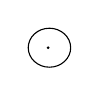
\begin{tikzpicture}[scale=.55]\draw (0,0) ellipse (.49 and .45);\fill (-.03,0) circle (.035);\end{tikzpicture}}
% archive sheet number: 14

\scanpage{16}
\mspage{A - 21 -}\hfill n$^{\mathrm o}$ 413

de $V$ dans $N$ comme étant un élément de $\operatorname{Hom}(U(\underline V);N)$ et noter $\widehat P(\underline V;N)$ le module ainsi défini, $\widehat P_+(\underline V;N)$ désignant le sous-module des applications linéaires nulles sur $U_0(\underline V)$. Ceci ne peut être gênant puisque dans le cas d'un module libre, il y a un isomorphisme canonique de l'un sur l'autre des deux modules notés $\widehat P_+(\underline V;N)$. Si $N=K$, on identifiera $\widehat P(\underline V;K)$ et $\widehat P(\underline V)$.

Soient $\underline V$ et $\underline W$ deux noyaux formels. Nous allons caractériser les applications linéaires de $U(\underline V)$ dans $U(\underline W)$ qui proviennent d'applications formelles de $\underline V$ dans $\underline W$ :

PROPOSITION 8.- \uline{Pour qu'une application linéaire} $\handwritten{\psi}$ \uline{de} $U(\underline V)$ \uline{dans} $U(\underline W)$ \uline{soit de la forme} $\varphi_*$ \uline{avec} $\varphi\in\widehat P_+(\underline V;\underline W)$, \uline{il faut et il suffit que} $\handwritten{\psi}(U_0(\underline V))=U_0(\underline W)$ \uline{et que} $\handwritten{\psi}$ \uline{soit compatible avec les applications diagonales} (\uline{c'est-à-dire que} $(\handwritten{\psi}\otimes\handwritten{\psi})\circ\Gamma=\Gamma\circ\handwritten{\psi}$).

Que les conditions soient nécessaires résulte de la prop. 6. La prop. 7 montre d'ailleurs que si $\varphi$ existe, elle est unique. Pour démontrer l'existence de $\varphi$, on se ramène en prenant des cartes formelles, au cas de noyaux formels définis par des modules libres $M$ et $N$. Soit alors $(e_i)_{i\in I}$ une base de $M$, $(e'_j)_{j\in J}$ une base de $M'$, et posons :
\[
\handwritten{\psi}(e_\alpha)=\sum a_{\alpha,\beta}\,e'_\beta \qquad(a_{\alpha,\beta}\in K).\tag*{(30)}
\]
La condition $\handwritten{\psi}(U_0(V))=U_0(W)$ entraîne
\[
a_{0,\beta}=0\quad\text{pour }|\beta|\geq 1\ ,\quad a_{0,0}\neq 0.\tag*{(31)}
\]
La compatibilité de $\handwritten{\psi}$ avec les applications diagonales donne :
\[
a_{\alpha,\beta_1+\beta_2}=\sum_{\alpha_1+\alpha_2=\alpha}a_{\alpha_1,\beta_1}\,a_{\alpha_2,\beta_2}.\tag*{(32)}
\]
% archive sheet number: 15

\scanpage{17}
\margin{faire le raisonnement}% slanted

Alors on voit que $P_{\mathrm{an}}(1_Y)$ est la classe de \unsure{Ch.|Coh.} sur $X-a$ représentée par la forme diff. $\frac{dz}{z}$, et par suite \deleted{\unsure{on a}} si $P_{\mathrm{an}}(1_Y)=\lambda P_{\mathrm{top}}(1_Y)$, on a
\[
\lambda=\underset{\substack{\nwarrow\qquad\nearrow\\\text{\inserted{cercle \unsure{centré|anti} \deleted{\unsure{cercle|en $a$}} orienté.}}}}{\int_C P_{\mathrm{an}}(1_Y)=\int_C\frac{dz}{z}}=2i\pi
\]

Donc
\[
\boxed{P_{\mathrm{an}}\left(\frac{1}{2i\pi}1_Y\right)=P_{\mathrm{top}}(1_Y)}
\]
\[
\boxed{\left\{\begin{aligned}
P_{\mathrm{top}}(1_Y)&=\frac{1}{2i\pi}P_{\mathrm{an}}(1_Y)\\
P_{\mathrm{an}}(1_Y)&=2i\pi\,P_{\mathrm{top}}(1_Y)
\end{aligned}\right.}
\]

\uline{\unsure{Cor.|Gys|Gén.|Ex.}} Considérons le diagramme
\diagram{\resizebox{\linewidth}{!}{\begin{tikzcd}[ampersand replacement=\&,row sep=large,column sep=large]
H_{\unsure{\alpha|a}}^{i+p}(X,\mathbb Z) \arrow[r,leftrightarrow] \& \unsure{H|\mathbb H}_{\deleted{\unsure{Z|Y}}}^{\deleted{\unsure{2|j}}i+p}(X,\mathbb C) \arrow[r,dash,"{\substack{\text{De Rham}\\\sim}}"] \& H^{\deleted{\unsure{2|j}}i+p}(X,\Omega_X^\bullet)\\
H_{\deleted{\unsure{Z|Y}}}^{i}(Y,\mathbb Z) \arrow[u,"{P_{\mathrm{top}}}"] \arrow[r] \& H_{\deleted{\unsure{Z|Y}}}^{\deleted{\unsure{2|j}}i}(\deleted{\unsure{X}}Y,\mathbb C) \arrow[u,"{P_{\mathrm{top}}}"] \arrow[r,dash,"{\substack{\deleted{\unsure{\text{De R.}}}\\\sim}}","{\frac{1}{(2i\pi)^p}\,\mathrm{can.}}"'] \& \underline{\underline H}_{\deleted{\unsure{Z|Y}}}^{i}(Y,\Omega^\bullet_Y) \arrow[u,"{P_{\mathrm{an}}}"]
\end{tikzcd}}}

\uline{Il est commutatif}, i.e. la formule ci-dessus est valable \uline{globalement}, et en remplaçant $1_Y$ par une classe de Coh. quelc. Provient de la comm. des
% archive sheet number: 16
